\documentclass[landscape]{article}
\usepackage[a4paper,margin=8mm]{geometry}
\usepackage{tikz}
\usepackage{amsmath}
\usepackage{graphicx}
\usetikzlibrary{arrows.meta,positioning,fit,decorations.pathreplacing,calc}
\pagestyle{empty}

\definecolor{inputblue}{HTML}{DDF1FA}
\definecolor{encodepurple}{HTML}{DCD6FF}
\definecolor{temporalorange}{HTML}{FFE4C6}
\definecolor{treegreen}{HTML}{DDF8D8}
\definecolor{denseyellow}{HTML}{FFF3BF}
\definecolor{graphcyan}{HTML}{DDF7F4}
\definecolor{outputblue}{HTML}{E8F5FA}
\definecolor{textdark}{HTML}{17202A}
\definecolor{linegray}{HTML}{6B7280}
\definecolor{stageblue}{HTML}{3B82F6}
\definecolor{stageorange}{HTML}{F59E0B}
\definecolor{stagegreen}{HTML}{22C55E}
\definecolor{stagepink}{HTML}{EC4899}

\tikzset{
  >=Latex,
  title/.style={font=\sffamily\bfseries\Large,text=textdark},
  subtitle/.style={font=\sffamily\small,text=linegray},
  tensor/.style={
    rectangle, rounded corners=3pt, draw=linegray, line width=0.8pt,
    minimum width=1.9cm, minimum height=1.15cm, align=center,
    font=\sffamily\small, text=textdark
  },
  layer/.style={
    rectangle, rounded corners=3pt, draw=linegray, line width=0.9pt,
    minimum width=2.15cm, minimum height=1.45cm, align=center,
    font=\sffamily\small, text=textdark
  },
  smalllayer/.style={
    rectangle, rounded corners=3pt, draw=linegray, line width=0.9pt,
    minimum width=1.8cm, minimum height=1.25cm, align=center,
    font=\sffamily\small, text=textdark
  },
  arrow/.style={-{Latex[length=2.6mm,width=1.8mm]}, line width=0.9pt, draw=linegray},
  stage/.style={font=\sffamily\scriptsize\bfseries},
  note/.style={font=\sffamily\scriptsize, text=linegray, align=center}
}

\newcommand{\figtitle}[2]{
  \node[title] at (0,2.95) {#1};
  \node[subtitle] at (0,2.52) {#2};
}

\newcommand{\stagebrace}[5]{
  \draw[#3, decorate, decoration={brace, amplitude=4pt}]
    ($(#1.north west)+(-0.05,0.27)$) -- ($(#2.north east)+(0.05,0.27)$)
    node[midway, yshift=0.34cm, stage, text=#3] {#4};
  \node[note] at ($(#1.south)!0.5!(#2.south)+(0,-0.72)$) {#5};
}

\begin{document}

\begin{center}
\resizebox{0.98\linewidth}{!}{
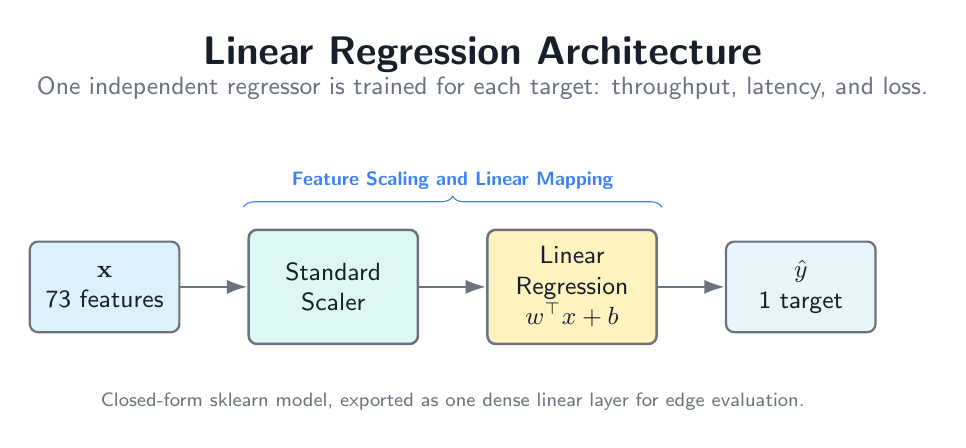
\begin{tikzpicture}[node distance=0.85cm]
\figtitle{Linear Regression Architecture}{One independent regressor is trained for each target: throughput, latency, and loss.}
\node[tensor, fill=inputblue] (in) at (-4.8,0) {$\mathbf{x}$\\73 features};
\node[layer, fill=graphcyan, right=of in] (scale) {Standard\\Scaler};
\node[layer, fill=denseyellow, right=of scale] (lin) {Linear\\Regression\\$w^\top x + b$};
\node[tensor, fill=outputblue, right=of lin] (out) {$\hat{y}$\\1 target};
\draw[arrow] (in) -- (scale);
\draw[arrow] (scale) -- (lin);
\draw[arrow] (lin) -- (out);
\stagebrace{scale}{lin}{stageblue}{Feature Scaling and Linear Mapping}{Closed-form sklearn model, exported as one dense linear layer for edge evaluation.}
\end{tikzpicture}}
\end{center}
\newpage

\begin{center}
\resizebox{0.98\linewidth}{!}{
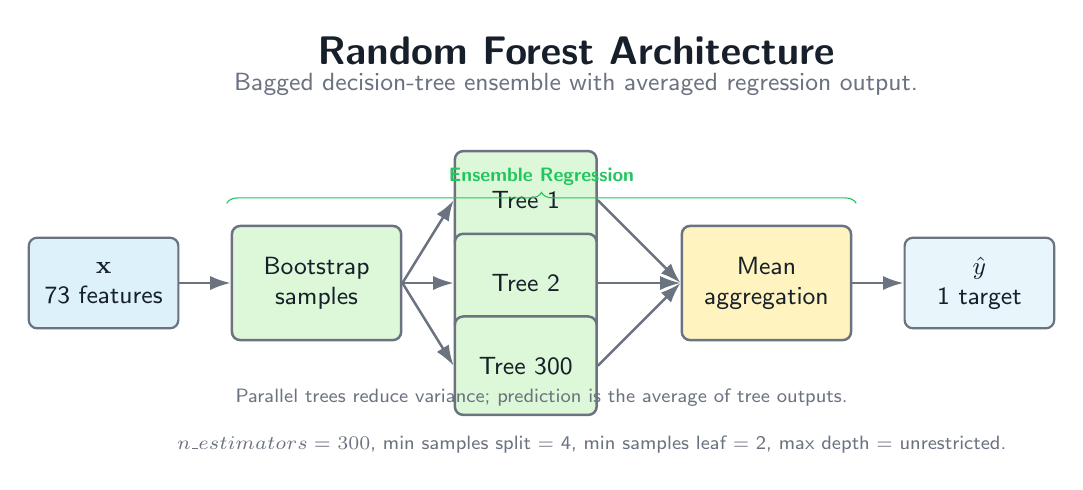
\begin{tikzpicture}[node distance=0.65cm]
\figtitle{Random Forest Architecture}{Bagged decision-tree ensemble with averaged regression output.}
\node[tensor, fill=inputblue] (in) at (-6.0,0) {$\mathbf{x}$\\73 features};
\node[layer, fill=treegreen, right=of in] (boot) {Bootstrap\\samples};
\node[smalllayer, fill=treegreen, right=of boot, yshift=1.05cm] (t1) {Tree 1};
\node[smalllayer, fill=treegreen, right=of boot] (t2) {Tree 2};
\node[smalllayer, fill=treegreen, right=of boot, yshift=-1.05cm] (t3) {Tree 300};
\node[layer, fill=denseyellow, right=1.05cm of t2] (avg) {Mean\\aggregation};
\node[tensor, fill=outputblue, right=of avg] (out) {$\hat{y}$\\1 target};
\draw[arrow] (in) -- (boot);
\draw[arrow] (boot.east) -- (t1.west);
\draw[arrow] (boot.east) -- (t2.west);
\draw[arrow] (boot.east) -- (t3.west);
\draw[arrow] (t1.east) -- (avg.west);
\draw[arrow] (t2.east) -- (avg.west);
\draw[arrow] (t3.east) -- (avg.west);
\draw[arrow] (avg) -- (out);
\node[note] at (0.2,-2.05) {$n\_estimators=300$, min samples split = 4, min samples leaf = 2, max depth = unrestricted.};
\stagebrace{boot}{avg}{stagegreen}{Ensemble Regression}{Parallel trees reduce variance; prediction is the average of tree outputs.}
\end{tikzpicture}}
\end{center}
\newpage

\begin{center}
\resizebox{0.98\linewidth}{!}{
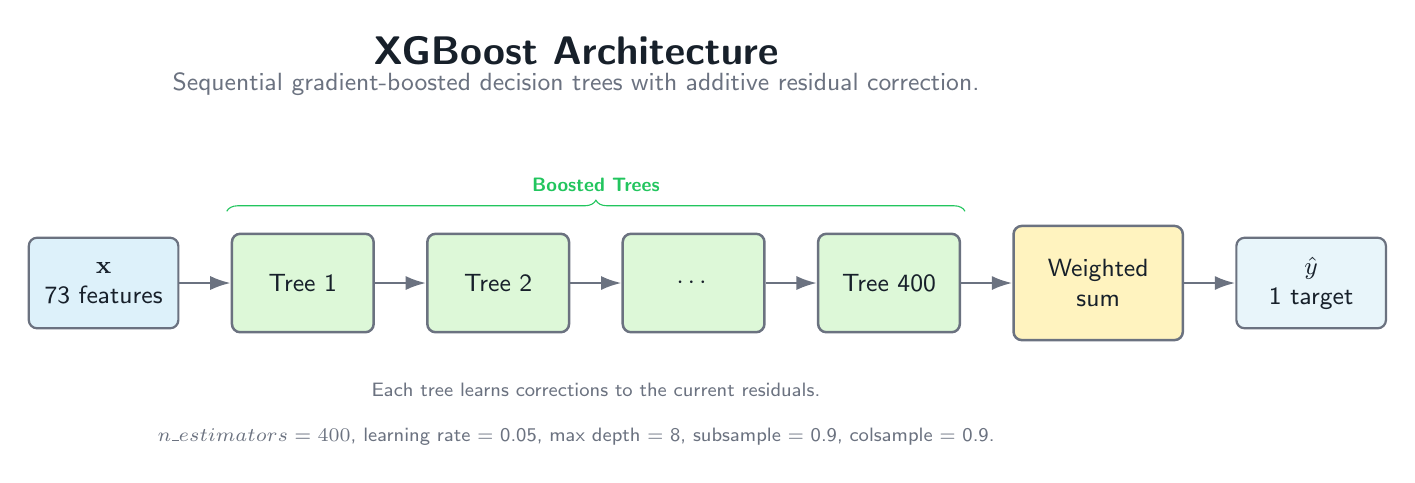
\begin{tikzpicture}[node distance=0.65cm]
\figtitle{XGBoost Architecture}{Sequential gradient-boosted decision trees with additive residual correction.}
\node[tensor, fill=inputblue] (in) at (-6.0,0) {$\mathbf{x}$\\73 features};
\node[smalllayer, fill=treegreen, right=of in] (t1) {Tree 1};
\node[smalllayer, fill=treegreen, right=of t1] (t2) {Tree 2};
\node[smalllayer, fill=treegreen, right=of t2] (td) {$\cdots$};
\node[smalllayer, fill=treegreen, right=of td] (t400) {Tree 400};
\node[layer, fill=denseyellow, right=of t400] (sum) {Weighted\\sum};
\node[tensor, fill=outputblue, right=of sum] (out) {$\hat{y}$\\1 target};
\draw[arrow] (in) -- (t1);
\draw[arrow] (t1) -- (t2);
\draw[arrow] (t2) -- (td);
\draw[arrow] (td) -- (t400);
\draw[arrow] (t400) -- (sum);
\draw[arrow] (sum) -- (out);
\node[note] at (0,-1.95) {$n\_estimators=400$, learning rate = 0.05, max depth = 8, subsample = 0.9, colsample = 0.9.};
\stagebrace{t1}{t400}{stagegreen}{Boosted Trees}{Each tree learns corrections to the current residuals.}
\end{tikzpicture}}
\end{center}
\newpage

\begin{center}
\resizebox{0.98\linewidth}{!}{
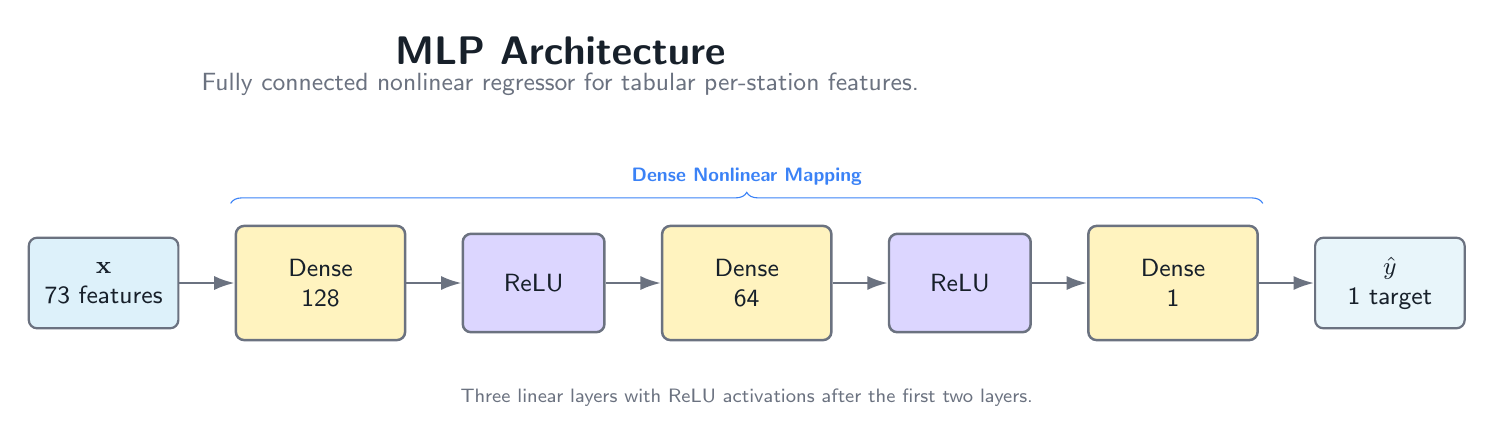
\begin{tikzpicture}[node distance=0.7cm]
\figtitle{MLP Architecture}{Fully connected nonlinear regressor for tabular per-station features.}
\node[tensor, fill=inputblue] (in) at (-5.8,0) {$\mathbf{x}$\\73 features};
\node[layer, fill=denseyellow, right=of in] (fc1) {Dense\\128};
\node[smalllayer, fill=encodepurple, right=of fc1] (r1) {ReLU};
\node[layer, fill=denseyellow, right=of r1] (fc2) {Dense\\64};
\node[smalllayer, fill=encodepurple, right=of fc2] (r2) {ReLU};
\node[layer, fill=denseyellow, right=of r2] (fc3) {Dense\\1};
\node[tensor, fill=outputblue, right=of fc3] (out) {$\hat{y}$\\1 target};
\draw[arrow] (in) -- (fc1);
\draw[arrow] (fc1) -- (r1);
\draw[arrow] (r1) -- (fc2);
\draw[arrow] (fc2) -- (r2);
\draw[arrow] (r2) -- (fc3);
\draw[arrow] (fc3) -- (out);
\stagebrace{fc1}{fc3}{stageblue}{Dense Nonlinear Mapping}{Three linear layers with ReLU activations after the first two layers.}
\end{tikzpicture}}
\end{center}
\newpage

\begin{center}
\resizebox{0.98\linewidth}{!}{
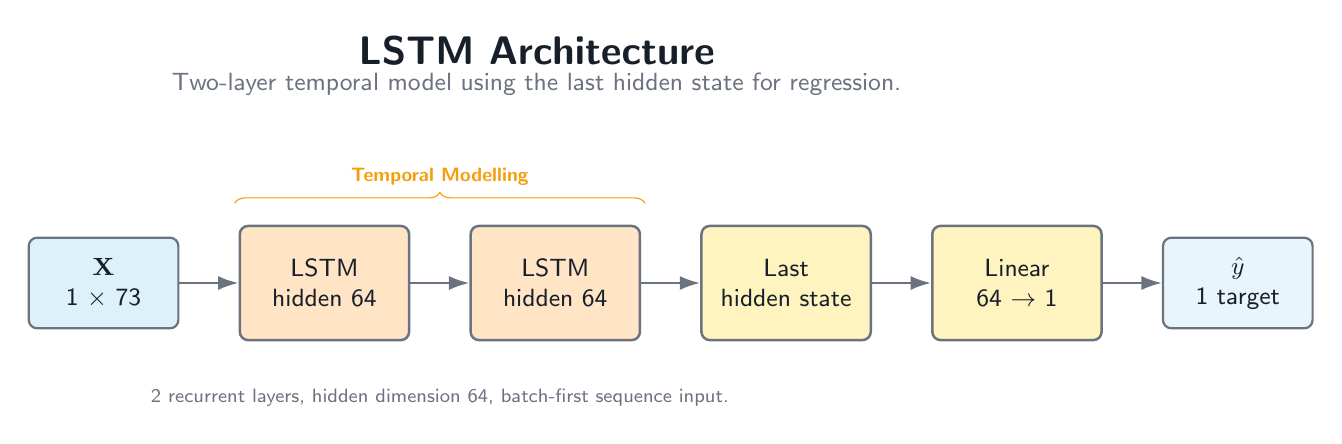
\begin{tikzpicture}[node distance=0.75cm]
\figtitle{LSTM Architecture}{Two-layer temporal model using the last hidden state for regression.}
\node[tensor, fill=inputblue] (in) at (-5.5,0) {$\mathbf{X}$\\1 $\times$ 73};
\node[layer, fill=temporalorange, right=of in] (l1) {LSTM\\hidden 64};
\node[layer, fill=temporalorange, right=of l1] (l2) {LSTM\\hidden 64};
\node[layer, fill=denseyellow, right=of l2] (last) {Last\\hidden state};
\node[layer, fill=denseyellow, right=of last] (fc) {Linear\\64 $\to$ 1};
\node[tensor, fill=outputblue, right=of fc] (out) {$\hat{y}$\\1 target};
\draw[arrow] (in) -- (l1);
\draw[arrow] (l1) -- (l2);
\draw[arrow] (l2) -- (last);
\draw[arrow] (last) -- (fc);
\draw[arrow] (fc) -- (out);
\stagebrace{l1}{l2}{stageorange}{Temporal Modelling}{2 recurrent layers, hidden dimension 64, batch-first sequence input.}
\end{tikzpicture}}
\end{center}
\newpage

\begin{center}
\resizebox{0.98\linewidth}{!}{
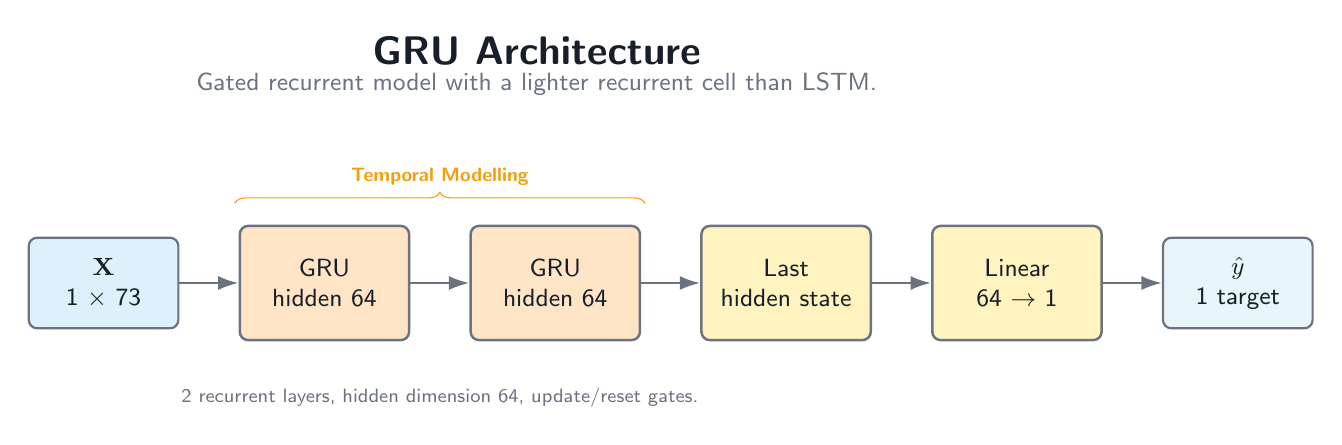
\begin{tikzpicture}[node distance=0.75cm]
\figtitle{GRU Architecture}{Gated recurrent model with a lighter recurrent cell than LSTM.}
\node[tensor, fill=inputblue] (in) at (-5.5,0) {$\mathbf{X}$\\1 $\times$ 73};
\node[layer, fill=temporalorange, right=of in] (g1) {GRU\\hidden 64};
\node[layer, fill=temporalorange, right=of g1] (g2) {GRU\\hidden 64};
\node[layer, fill=denseyellow, right=of g2] (last) {Last\\hidden state};
\node[layer, fill=denseyellow, right=of last] (fc) {Linear\\64 $\to$ 1};
\node[tensor, fill=outputblue, right=of fc] (out) {$\hat{y}$\\1 target};
\draw[arrow] (in) -- (g1);
\draw[arrow] (g1) -- (g2);
\draw[arrow] (g2) -- (last);
\draw[arrow] (last) -- (fc);
\draw[arrow] (fc) -- (out);
\stagebrace{g1}{g2}{stageorange}{Temporal Modelling}{2 recurrent layers, hidden dimension 64, update/reset gates.}
\end{tikzpicture}}
\end{center}
\newpage

\begin{center}
\resizebox{0.98\linewidth}{!}{
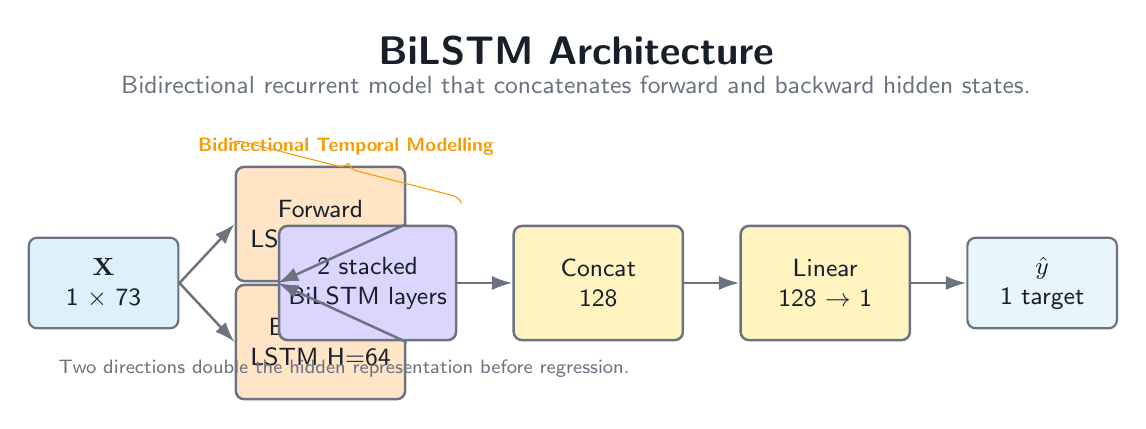
\begin{tikzpicture}[node distance=0.7cm]
\figtitle{BiLSTM Architecture}{Bidirectional recurrent model that concatenates forward and backward hidden states.}
\node[tensor, fill=inputblue] (in) at (-6.0,0) {$\mathbf{X}$\\1 $\times$ 73};
\node[layer, fill=temporalorange, right=of in, yshift=0.75cm] (fw) {Forward\\LSTM H=64};
\node[layer, fill=temporalorange, right=of in, yshift=-0.75cm] (bw) {Backward\\LSTM H=64};
\node[layer, fill=encodepurple, right=1.25cm of in] (stack) {2 stacked\\BiLSTM layers};
\node[layer, fill=denseyellow, right=of stack] (cat) {Concat\\128};
\node[layer, fill=denseyellow, right=of cat] (fc) {Linear\\128 $\to$ 1};
\node[tensor, fill=outputblue, right=of fc] (out) {$\hat{y}$\\1 target};
\draw[arrow] (in.east) -- (fw.west);
\draw[arrow] (in.east) -- (bw.west);
\draw[arrow] (fw.east) -- (stack.west);
\draw[arrow] (bw.east) -- (stack.west);
\draw[arrow] (stack) -- (cat);
\draw[arrow] (cat) -- (fc);
\draw[arrow] (fc) -- (out);
\stagebrace{fw}{stack}{stageorange}{Bidirectional Temporal Modelling}{Two directions double the hidden representation before regression.}
\end{tikzpicture}}
\end{center}
\newpage

\begin{center}
\resizebox{0.98\linewidth}{!}{
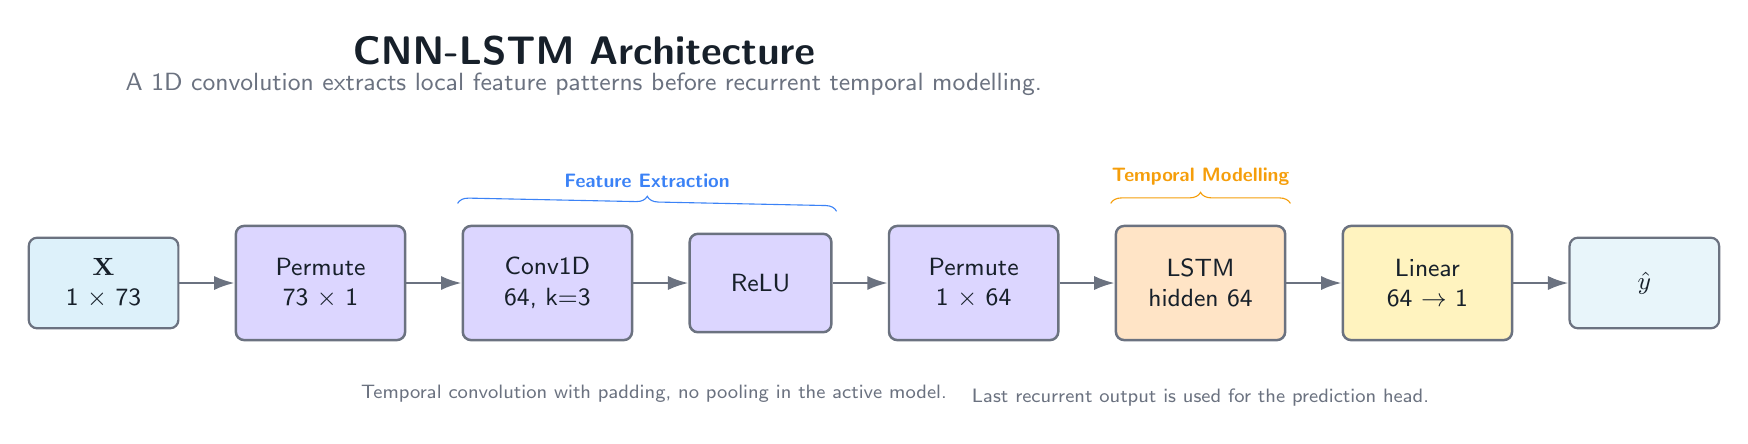
\begin{tikzpicture}[node distance=0.7cm]
\figtitle{CNN-LSTM Architecture}{A 1D convolution extracts local feature patterns before recurrent temporal modelling.}
\node[tensor, fill=inputblue] (in) at (-6.1,0) {$\mathbf{X}$\\1 $\times$ 73};
\node[layer, fill=encodepurple, right=of in] (perm1) {Permute\\73 $\times$ 1};
\node[layer, fill=encodepurple, right=of perm1] (conv) {Conv1D\\64, k=3};
\node[smalllayer, fill=encodepurple, right=of conv] (relu) {ReLU};
\node[layer, fill=encodepurple, right=of relu] (perm2) {Permute\\1 $\times$ 64};
\node[layer, fill=temporalorange, right=of perm2] (lstm) {LSTM\\hidden 64};
\node[layer, fill=denseyellow, right=of lstm] (fc) {Linear\\64 $\to$ 1};
\node[tensor, fill=outputblue, right=of fc] (out) {$\hat{y}$};
\draw[arrow] (in) -- (perm1);
\draw[arrow] (perm1) -- (conv);
\draw[arrow] (conv) -- (relu);
\draw[arrow] (relu) -- (perm2);
\draw[arrow] (perm2) -- (lstm);
\draw[arrow] (lstm) -- (fc);
\draw[arrow] (fc) -- (out);
\stagebrace{conv}{relu}{stageblue}{Feature Extraction}{Temporal convolution with padding, no pooling in the active model.}
\stagebrace{lstm}{lstm}{stageorange}{Temporal Modelling}{Last recurrent output is used for the prediction head.}
\end{tikzpicture}}
\end{center}
\newpage

\begin{center}
\resizebox{0.98\linewidth}{!}{
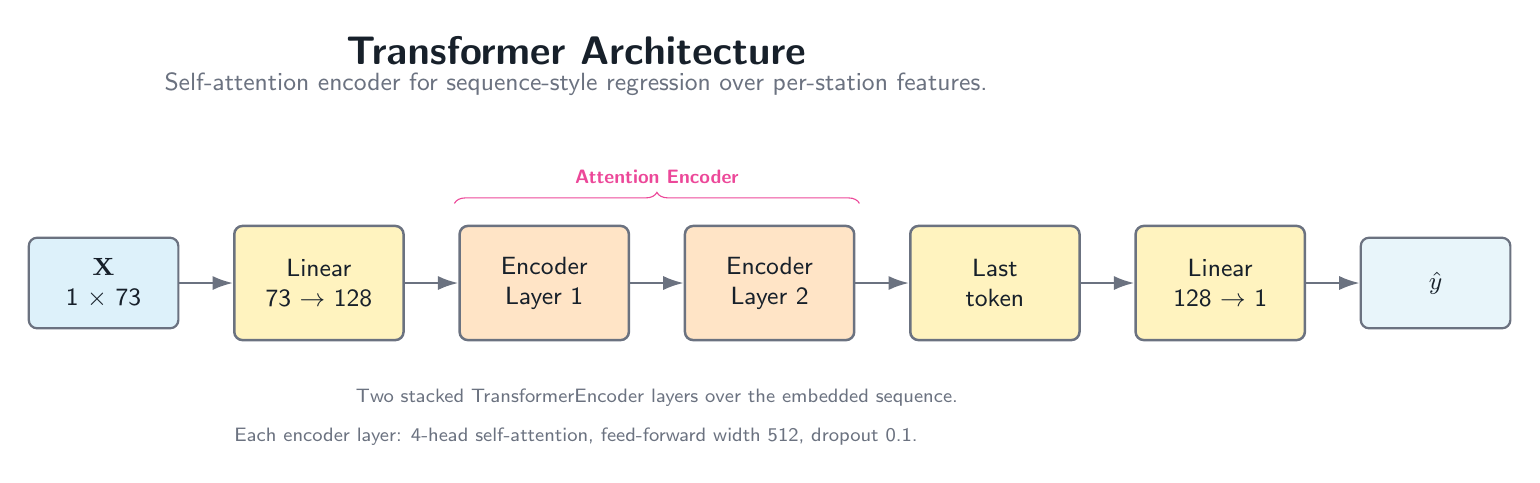
\begin{tikzpicture}[node distance=0.68cm]
\figtitle{Transformer Architecture}{Self-attention encoder for sequence-style regression over per-station features.}
\node[tensor, fill=inputblue] (in) at (-6.0,0) {$\mathbf{X}$\\1 $\times$ 73};
\node[layer, fill=denseyellow, right=of in] (emb) {Linear\\73 $\to$ 128};
\node[layer, fill=temporalorange, right=of emb] (enc1) {Encoder\\Layer 1};
\node[layer, fill=temporalorange, right=of enc1] (enc2) {Encoder\\Layer 2};
\node[layer, fill=denseyellow, right=of enc2] (last) {Last\\token};
\node[layer, fill=denseyellow, right=of last] (fc) {Linear\\128 $\to$ 1};
\node[tensor, fill=outputblue, right=of fc] (out) {$\hat{y}$};
\draw[arrow] (in) -- (emb);
\draw[arrow] (emb) -- (enc1);
\draw[arrow] (enc1) -- (enc2);
\draw[arrow] (enc2) -- (last);
\draw[arrow] (last) -- (fc);
\draw[arrow] (fc) -- (out);
\node[note] at (0,-1.95) {Each encoder layer: 4-head self-attention, feed-forward width 512, dropout 0.1.};
\stagebrace{enc1}{enc2}{stagepink}{Attention Encoder}{Two stacked TransformerEncoder layers over the embedded sequence.}
\end{tikzpicture}}
\end{center}
\newpage

\begin{center}
\resizebox{0.98\linewidth}{!}{
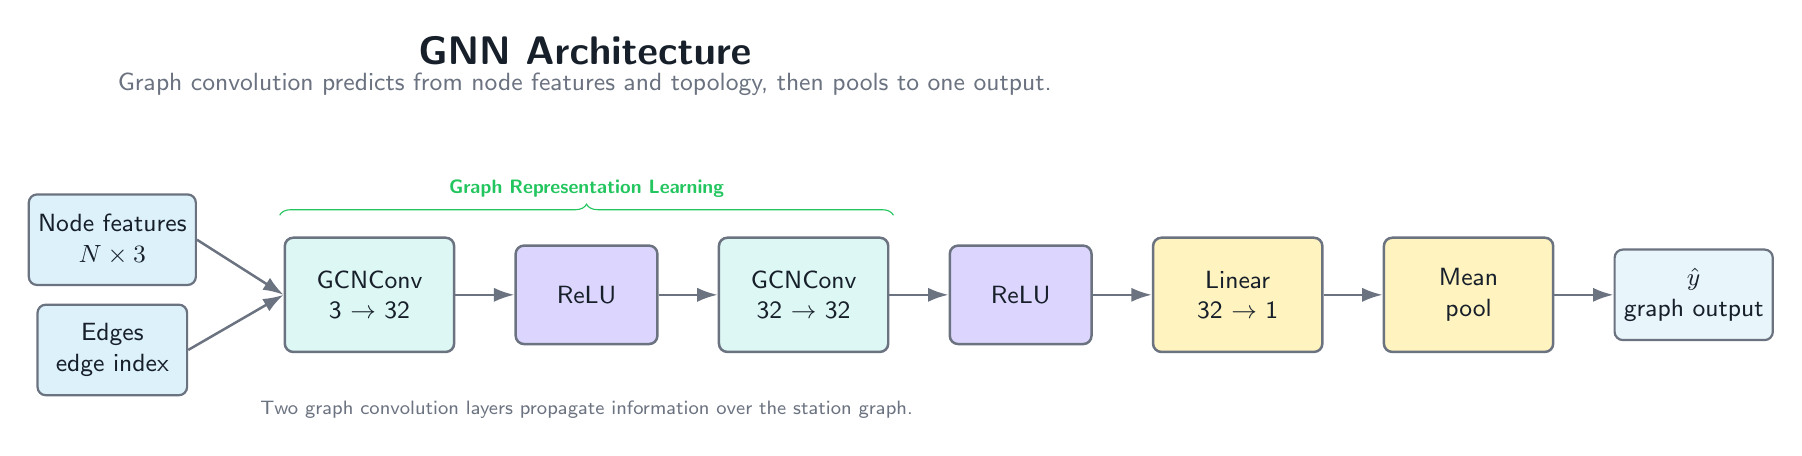
\begin{tikzpicture}[node distance=0.75cm]
\figtitle{GNN Architecture}{Graph convolution predicts from node features and topology, then pools to one output.}
\node[tensor, fill=inputblue] (x) at (-6.0,0.55) {Node features\\$N \times 3$};
\node[tensor, fill=inputblue] (e) at (-6.0,-0.85) {Edges\\edge index};
\node[layer, fill=graphcyan, right=1.1cm of x, yshift=-0.7cm] (g1) {GCNConv\\3 $\to$ 32};
\node[smalllayer, fill=encodepurple, right=of g1] (r1) {ReLU};
\node[layer, fill=graphcyan, right=of r1] (g2) {GCNConv\\32 $\to$ 32};
\node[smalllayer, fill=encodepurple, right=of g2] (r2) {ReLU};
\node[layer, fill=denseyellow, right=of r2] (fc) {Linear\\32 $\to$ 1};
\node[layer, fill=denseyellow, right=of fc] (pool) {Mean\\pool};
\node[tensor, fill=outputblue, right=of pool] (out) {$\hat{y}$\\graph output};
\draw[arrow] (x.east) -- (g1.west);
\draw[arrow] (e.east) -- (g1.west);
\draw[arrow] (g1) -- (r1);
\draw[arrow] (r1) -- (g2);
\draw[arrow] (g2) -- (r2);
\draw[arrow] (r2) -- (fc);
\draw[arrow] (fc) -- (pool);
\draw[arrow] (pool) -- (out);
\stagebrace{g1}{g2}{stagegreen}{Graph Representation Learning}{Two graph convolution layers propagate information over the station graph.}
\end{tikzpicture}}
\end{center}

\end{document}
